%-*- coding: UTF-8 -*-
\documentclass[UTF8]{ctexart}
\usepackage{geometry}
\geometry{a4paper,centering,scale=0.8}
\usepackage{graphicx}
\usepackage{amsmath}
\usepackage{textcomp}
\usepackage{amsthm}
\usepackage{amssymb}

\title{\heiti Machine Learning}
\author{卢婧宇}

\begin{document}
\maketitle
\tableofcontents

\newpage
\section{Introduction}
\subsection{Welcome}
 第一个视频主要讲了什么是机器学习,机器学习能做什么。
\begin{itemize}
  \item Grew out of work AI

  \item New capability for computers
\end{itemize}

 机器学习的案例:
\begin{itemize}
  \item Database mining 数据挖掘

    Large datasets from growth of automation/web

    E.g.,Web click data 点击数据流, medical records, biology, engineering

  \item Applications can't program by hand.

    E.g.,Autonomous helicopter, handwriting recognition, most of Natural Language Processing(NLP), Computer Vision
  \item Self-customizing programs 自定制程序

   E.g., Amazon, Netflix product recommendations
\end{itemize}
\subsection{What is Machine Learning?}
第一个机器学习的定义来自于 Arthur Samuel。他定义机器学习为,在不进行特定编程的情况下,给予计算机 学习能力的领域。

另一个年代近一点的定义,Tom Mitchell 定义的机器学习是,一个好的学 习问题定义如下,他说,一个程序被认为能从经验 E 中学习,解决任务 T,
达到性能度量值 P,当且仅当,有了经验 E 后,经过 P 评判,程序在处理 T 时的性能有所提升。

Example: playing checkers.

E = the experience of playing many games of checkers

T = the task of playing checkers.

P = the probability that the program will win the next game.

目前存在几种不同类型的学习算法。主要的两种类型被我们称之为监督学习(supervised learning)和无监督学习(unsupervised learning)。
其他的有,强化学习(Reinforcement learning), 推荐系统(recommender systems)。也会提到应用学习算法的实用建议(Practical advice for applying learning algorithms)。
\subsection{Intorduction Supervised Learning 介绍监督学习}
Supervised Learning ``right answers''given.监督学习指的就是我们给学习算法一个数据集,这个数据集由``正确答案''组成。(售楼的例子中事先获取到的准确数据)
用术语来讲,这叫做回归问题。回归(regression)这个词的意思是,我们在试着推测出这一系列连续值属性(Predict continuous valued output)。

肿瘤样本的例子属于分类问题,其目标是推出一组离散结果。实际的分类问题中输出会不止两个值。预测肿瘤的恶性与否用到的特征,在机器学习问题中,可能会遇到不止一种特征。如果想用无限多种特征好让你的算法可以利用大量的特征,
或者说线索来做推测。如何处理怎么存出这些特征都存在问题,电脑内存会不够。用支持向量机来解决,可以让计算计处理无限多个特征。
\subsection{Intorduction Unsupervised Learning 介绍无监督学习}
无监督学习中的数据没有任何标签或者是有相同的标签或者就是没标签,没有基于预测结果的反馈。但无监督学习算法可能会把这些数据分成不同的簇,叫做聚类算法(clustering)。

无监督学习或者聚类算法在其他领域有着大量应用:组织大型的计算机群(organize computing clusters)、社交网络分析(social network analysis)、
市场分割中的应用(market segmentation)、天文数据分析(astronomical data analysis)。这些都是聚类的例子,聚类只是无监督学习的一种。
基因问题,找到一种方法,将这些基因自动组合成类似或相关的不同变量,如寿命、位置、角色等。

另一种非聚类问题,鸡尾酒宴问题,允许你在混乱的环境中找到结构。就是从重叠的音频中分离音频。代码:

[W, s, v] = svd ((repmat(sum(x.$*$x,1),size(x,1),1).$*$x)$*$x');

\section{Linear Regression with One Variable 单变量线性回归}
\subsection{Model Representation 模型表示}
对于监督学习,第一个学习的算法是线性回归算法(Linear regression)。例子是预测住房价格,是回归问题,回归指的是根据之前的数据预测出一个准确的输出值。另一种最常见的监督学习方式,叫做分类问题。例子是肿瘤问题,
想要预测离散的输出值。更进一步来说,在监督学习中我们有一个数据集,这个数据集被称为训练集。
以房屋交易问题为例如图 ~\ref{fig:2} 所示。
\begin{figure}[htb]
 \center{\includegraphics[width=10cm]  {house.jpg}}
 \caption{房屋交易数据}
 \label{fig:2}
 \end{figure}

 描述这个回归问题的标记如下:
\begin{itemize}
  \item $m$ = Number of training examples
  \item $x$ = ``intput''variable / features
  \item $y$ = ``output''variable / ``target''variable
  \item ($x,y$) = one training example
  \item ($x^{(i)},y^{(i)}$) = i training example
\end{itemize}

监督学习算法的工作方式,如图 ~\ref{fig:1} 所示:

训练集(Training Set)输入 学习算法(Learning Algorithm) 输出  函数h(hypothesis假设)

h 根据 输入的x 得到 输出y

\begin{figure}[htb]
 \center{\includegraphics[width=9cm]  {监督学习工作方式.jpg}}
 \caption{监督学习算法的工作方式}
 \label{fig:1}
 \end{figure}

因此,h是一个从x到y的函数映射。如何表达h?一种可能表达方式为:$h_\theta(x)=\theta_0+\theta_1x$,因为只含有一个特征/输入变量,因此这样的问题叫做单变量线性回归问题。

\subsection{Cost Function 代价函数}
如何把最有可能的直线与我们的数据相拟合?$\theta_i$ 称为模型参数,所以就是要求$\theta_0$和$\theta_1$。
选择不同的参数会得到不同的假设h。Idea:Choose $\theta_0$,$\theta_1$ so that $h_\theta(x)$ is close to $y$ for our training examples($x,y$).
也就是说要解决的是一个最小化问题,写出关于$\theta_0$,$\theta_1$ 的最小化,而且希望这个式子极其小,想要h(x)和y之间的差异要小,
要做的事情是尽量减少假设的输出与房子真实价格之间的差的平方。

数学表达:

\begin{equation*}
  \min_{\theta_0 \theta_1}
  \frac{1}{2m}
  \sum^m_{\substack{i=1}}
   \Big(h_\theta(x^{(i)})-y^{(i)}\Big)^{2}
\end{equation*}

其中$h_\theta(x^{(i)})=\theta_0+\theta_1x^{(i)}$
我们实际上考虑的是这个数的1/m,因此我们要尝试尽量减少我们的平均误差,也就是尽量减少其1/2m,通常是这个数的一半。
前面的这些只是为了使数学更直白一点,因此对这个求和值的二分之一求最小值。
\begin{equation*}
  J(\theta_0,\theta_1)=
  \frac{1}{2m}
  \sum^m_{\substack{i=1}}
   \Big(h_\theta(x^{(i)})-y^{(i)}\Big)^{2}
\end{equation*}

J($\theta_0,\theta_1$)求最小值,就是代价函数,也被称为平方误差函数(squared error faction),有时也被称为平方误差代价函数。
我们之所以要求出误差的平方和,是因为误差平方代价函数对于大多数问题,特别是回归问题,都是一个合理的选择。还有其他的代价函数也能很好地发挥作用,
但是平方误差代价函数可能是解决回归问题最常用的手段了。

\subsection{Cost Function - Intuition 1 代价函数的直观理解1}
上一小节理解了代价函数的数学上的定义,本小结通过例子来获取一些直观的感受。
\newline

Hypothesis:
\begin{equation*}
    h_\theta(x)=\theta_0+\theta_1x
\end{equation*}

 Parameters:
\begin{equation*}
\theta_0,\theta_1
\end{equation*}

Cost Function:

\begin{equation*}
  J(\theta_0,\theta_1)=
  \frac{1}{2m}
  \sum^m_{\substack{i=1}}
   \Big(h_\theta(x^{(i)})-y^{(i)}\Big)^{2}
\end{equation*}

Goal:

\begin{equation*}
  \min_{\theta_0 \theta_1}
  J(\theta_0,\theta_1)
\end{equation*}

先把$\theta_0$设为0,所以现在就只有一个参数$\theta_1$,$h(x)=\theta_1x$,优化目标是$J(\theta_1)$
最小化。我们可以试着更好地理解代价函数这个概念,我们要理解的是这两个重要的函数,第一个是假设函数,第二个是代价函数。
注意这个假设函数 h(x),对于一个固定的$\theta_1$这是一个关于 x 的函数,所以这个假设函数就是一个关于 x 这个房子大小的函数。
与此不同的是代价函数 J 是一个关于参数$\theta_1$的函数,而$\theta_1$控制着这条直线的斜率,现在我们把这写函数都画出来,如图 ~\ref{fig:3} 所示。
我们从假设函数开始,比如说这里是我的训练样本,它包含了三个点 (1,1) (2,2) 和 (3,3) 。
\begin{figure}[htb]
 \center{\includegraphics[width=12cm]  {paint.jpg}}
 \caption{两种函数坐标图}
 \label{fig:3}
\end{figure}

对应将$\theta_1$取不同值得到的结果可以发现,当$\theta_1=1$时,代价函数最小。

\subsection{Cost Function - Intuition 2 代价函数的直观理解2}
本小结将更深入地学习代价函数的作用,现在是有两个参数起作用了,对于选取不同的值我们得到的结果如下图 ~\ref{fig:4} 所示。
\begin{figure}[htb]
 \center{\includegraphics[width=12cm]  {paint22.jpg}}
 \caption{两种函数坐标图}
 \label{fig:4}
\end{figure}

我们会遇到更复杂、更高维度、更多参数的情况,而这些情况是很难画出图的,因此更无法将其可视化,
因此我们真正需要的是编写程序来找出这些最小化代价函数的 $\theta_0$ 和 $\theta_1$ 的值,
在下一节中,将介绍一种算法,能够自动地找出能使代价函数 J最小化的参数 $\theta_0$ 和 $\theta_1$ 的值。
\subsection{Gradient Descent 梯度下降}
我们已经定义了代价函数J,而本结介绍梯度下降这种算法,这种算法可以将代价函数J最小化。
梯度下降是很常用的算法,它不仅被用在线性回归上,它实际上被广泛的应用于机器学习领域中的众多领域。
在后面课程中,为了解决其他线性回归问题,也将使用梯度下降法最小化其他函数,而不仅仅是只用在本节课的代价函数J。

例:


Have some function : J($\theta_0$,$\theta_1$) \quad J($\theta_0$,.....,$\theta_n$)

也许这是一个线性回归的代价函数,也许是一些其他函数。

Want : \begin{equation*}
  \min_{\theta_0 \theta_1}
  J(\theta_0,\theta_1)
\end{equation*}
\begin{equation*}
  \min_{\theta_0 .... \theta_n}
  J(\theta_0,.....,\theta_n)
\end{equation*}

要使其最小化,我们需要用一个算法,来最小化函数J($\theta_0$,$\theta_1$)。用n个$\theta$是为了证明梯度下降算法可以解决更一般的问题,但为了简洁只用两个参数。

Outline:
\begin{itemize}
 \item Start with some $\theta_0$,$\theta_1$
 \item Keep changing $\theta_0$,$\theta_1$ to reduce J($\theta_0$,$\theta_1$)
       until we hopefully end up at a minimum
\end{itemize}

如图 ~\ref{fig:5} 所示,为梯度下降法的工作原理。坐标轴 $\theta_0$ 和 $\theta_1$ 在水平轴上,而函数J在垂直坐标轴上,图形表面高度则是J的值。
我们希望最小化这个函数,所以我们从 $\theta_0$ 和 $\theta_1$ 的某个值出发。所以对 $\theta_0$ 和 $\theta_1$ 赋以某个初值,也就是对应于从这个函数表面上的某个起始点出发。
将这两个参数初始化为0。把找最小值问题看成下山问题,从山顶某一点寻找尽快下山的下一个点,就是找局部最优解。
\begin{figure}[htb]
 \center{\includegraphics[width=12cm]  {mountn.jpg}}
 \caption{梯度下降算法定义图}
 \label{fig:5}
\end{figure}

这个图是梯度下降算法的定义,我们将会反复做这些直到收敛。更新参数$\theta_j$的方法是用$\theta_j$减去$\alpha$乘以这一部分。

公式:

\begin{equation*}
  \theta_j := \theta_j - \alpha
  \frac{\partial}{\partial\theta_j}
  J(\theta_0,\theta_1)   \quad  (for \quad j=0 \quad and \quad j=1)
\end{equation*}

其中符号 := 表示赋值,$\alpha$是一个数字被称为学习速率。在梯度下降算法中,它控制了我们下山时会迈出多大的步子。
因此如果$\alpha$值很大,那么相应的梯度下降过程中,我们会试图用大步子下山,如果$\alpha$值很小,那么我们会迈着很小的小碎步下山。
关于如何设置$\alpha$的值等内容,在之后的课程中会详细说明。

关于如何更新$\theta_0$ 和 $\theta_1$的公式:

Correct:Simultaneous update

\begin{equation*}
  temp 0 := \theta_0 - \alpha
  \frac{\partial}{\partial\theta_0}
  J(\theta_0,\theta_1)
\end{equation*}
\begin{equation*}
  temp 1 := \theta_1 - \alpha
  \frac{\partial}{\partial\theta_1}
  J(\theta_0,\theta_1)
\end{equation*}
\begin{equation*}
  \theta_0 := temp 0
\end{equation*}
\begin{equation*}
\theta_1 := temp 1
\end{equation*}

注意是同时更新,而不是先更新$\theta_0$ ,将$\theta_0$ 带入$\theta_1$表达式再求$\theta_1$。
实际上同步更新是更自然的实现方法,当人们谈到梯度下降时他们的意思就是同步更新。如果用非同步更新去实现算法,代码可能也会正确工作,
但是并不是人们所指的那个梯度下降算法,而是具有不同性质的其他算法。由于各种原因,这其中会表现出微小的差别。

\subsection{Gradient Descent Intuition 梯度下降的直观理解}
上一节给出了一个数学上关于梯度下降的定义。本节我们更深入研究一下,更直观地感受一下这个算法是做什么的,以及梯度下降算法的更新过程有什么意义。

假设函数关于$\theta_1$的函数J,表达式及图像如下图 ~\ref{fig:6} 所示。

\begin{figure}[htb]
 \center{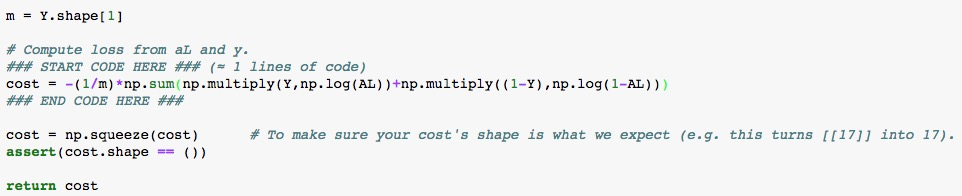
\includegraphics[width=10cm]  {6.jpg}}
 \caption{函数及图像}
 \label{fig:6}
\end{figure}

参数初始化到右边这点时,导数值为正,结果$\theta_1$变小向左移动。初始化在左边时,导数值为负,结果$\theta_1$变大向右移动。
当导数值为零时,参数值已经处于局部最低点,不会改变参数值。这也解释了为什么即使学习速率$\alpha$保持不变时,梯度下降也可以收敛到局部最低点。
\newline

再看$\alpha$对结果的影响:
\begin{itemize}
  \item If $\alpha$ is too small,gradient descent can be slow.
  \item If $\alpha$ is too large,gradient descent can overshoot
\end{itemize}

在梯度下降法中,当我们接近局部最低点时,梯度下降法会自动采取更小的幅度。这是因为当我们接近局部最低点时,很显然在局部最低时导数等于零。
所以当我们接近局部最低时,导数值会自动变得越来越小。所以梯度下降将自动采取较小的幅度,这就是梯度下降的做法,所以实际上没有必要再另外减小$\alpha$,这就是梯度下降算法。
可以用它来最小化任何代价函数J,不只是线性回归中的代价函数J。

\subsection{Gradient Descent For Linear Regression 梯度下降的线性回归}
在之前谈到关于梯度下降算法,梯度下降是很常用的算法,它不仅被用在线性回归上和线性回归模型、平方误差代价函数。本小结要将梯度下降和代价函数结合。
将用到此算法,并将其应用于具体的拟合直线的线性回归算法里。

梯度下降算法和线性回归算法比较如图 ~\ref{fig:7} 所示。
\begin{figure}[htb]
 \center{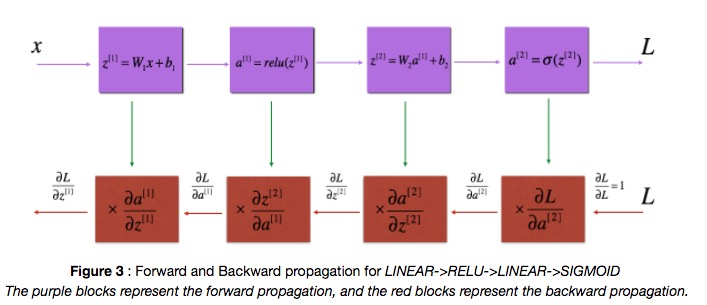
\includegraphics[width=13cm]  {7.jpg}}
 \caption{梯度下降算法和线性回归算法}
 \label{fig:7}
\end{figure}

对之前的线性回归问题运用梯度下降法,关键在于求出代价函数的导数:

\begin{equation*}
    \frac{\partial}{\partial\theta_j}
    J(\theta_0,\theta_1)=
    \frac{\partial}{\partial\theta_j}
    \frac{1}{2m}
    \sum^m_{\substack{i=1}}
     \Big(h_\theta(x^{(i)})-y^{(i)}\Big)^{2}
\end{equation*}

\begin{equation*}
    j=0 时: \quad \frac{\partial}{\partial\theta_0}
    J(\theta_0,\theta_1)=
    \frac{1}{m}
    \sum^m_{\substack{i=1}}
     \Big(h_\theta(x^{(i)})-y^{(i)}\Big)
\end{equation*}

\begin{equation*}
    j=1 时: \quad \frac{\partial}{\partial\theta_0}
    J(\theta_0,\theta_1)=
    \frac{1}{m}
    \sum^m_{\substack{i=1}}
     \Big(h_\theta(x^{(i)})-y^{(i)}\Big)\cdot x^{(i)}
\end{equation*}

则算法改写为:

Repeat until convergence,update $\theta_0$ and $\theta_1$ simultaneously :

 \begin{equation*}
  \theta_0:= \theta_0 - \alpha
  \frac{1}{m}
    \sum^m_{\substack{i=1}}
     \Big(h_\theta(x^{(i)})-y^{(i)}\Big)
\end{equation*}

\begin{equation*}
  \theta_1:= \theta_1 - \alpha
  \frac{1}{m}
    \sum^m_{\substack{i=1}}
     \Big(h_\theta(x^{(i)})-y^{(i)}\Big)\cdot x^{(i)}
\end{equation*}

这种算法也称为批量梯度下降(batch gradient descent。这些微分项实际上就是代价函数J的斜率。反复执行括号中的式子直到收敛,$\theta_0$ 和 $\theta_1$ 不断被更新,都是加上一个 $-\alpha/m$ 乘上后面的求和项,这就是我们的线性回归算法

执行梯度下降时有一个细节要注意,就是必须要同时更新$\theta_0$ 和 $\theta_1$。用梯度下降解决问题的一个原因是,它更容易得到局部最优值。根据你的初始化,你会得到不同的局部最优解。
事实证明用于线性回归的代价函数总是一个弓形,是一个凸函数(convex function)。它就是一个弓形的函数,因此这个函数没有任何局部最优解,只有一个全局最优解。
并且无论什么时候 你对这种代价函数使用线性回归梯度下降法得到的结果,总是收敛到全局最优值,因为没有全局最优以外的其他局部最优点。通常来说,初始化参数$\theta_0$ 和 $\theta_1$都为零。

\section{Linear Algebra Review 线性代数回顾}
\subsection{Matrices and Vector 矩阵和向量}
m行n列的矩阵$R^{nm}$:

\begin{equation*}
  \begin{bmatrix}
    p_{11} & p_{12} & \ldots & p_{1n} \\
    p_{21} & p_{22} & \ldots & p_{2n} \\
    \vdots & \vdots & \ddots & \vdots \\
    p_{m1} & p_{m2} & \ldots & p_{mn} \\
  \end{bmatrix}
\end{equation*}

矩阵的维数(Dimension of matrix)=行数(number of rows)$\times$列数(number of columns)

矩阵元素(Matrix Elements)(矩阵项 entries of matrix):$A_{ij}$指第i行,第j列的元素。

向量是一种特殊的矩阵,n维向量:

Vector:An n$\times$1 matrix
\begin{equation*}
  \begin{bmatrix}
    p_{1}  \\
    p_{2}  \\
    \vdots  \\
    p_{n}  \\
  \end{bmatrix}
\end{equation*}

元素表示:$y_{i}=i^{th}$element。如何引用向量元素:

1-indexed vs 0-indexed:

\begin{equation*}
 y=
  \begin{bmatrix}
    y_{1}  \\
    y_{2}  \\
    y_{3} \\
    y_{4}  \\
  \end{bmatrix} \qquad
  y=
   \begin{bmatrix}
     y_{0}  \\
     y_{1}  \\
     y_{2} \\
     y_{3}  \\
   \end{bmatrix}
\end{equation*}

事实上,在数学中1-索引的情况比较多,而对于很多机器学习的应用问题来说,0-索引向量为我们提供了一个更方便的符号表达。
使用 大写字母 如 A B C X 来表示矩阵,通常我使用小写字母像a b x y ,来表示数字、原始的数字、标量或向量。
但也会使用y来代表向量。

\subsection{Addition and Scalar Multiplical 加法和标量乘法}
矩阵的加法:行列数相等的可以加。

矩阵的乘法:每个元素都要乘。
\subsection{Matrix Vector Multiplication 矩阵向量乘法}

矩阵和向量的乘法如图:m×n 的矩阵乘以 n$\times$1 的向量,得到的是 m$\times$1 的向量。

举个例子,当你有四间房子,你想使用自己的预测函数来预测房子的价格完成这些工作:

House sizes: 2104 1416 1534 852

\begin{equation*}
h_\theta(x)=-40+0.25x
\end{equation*}

\begin{equation*}
  \begin{bmatrix}
    1 &  2104 \\
    1 &  1416  \\
    1 &  1534 \\
    1 &  852 \\
  \end{bmatrix} \quad \times \quad
  \begin{bmatrix}
     -40 \\
     0.25
  \end{bmatrix}
\end{equation*}

可以只写一行代码就完成整个过程,可以这样写: prediction = DataMatrix $\times$ Parameters 。

当有很多房子时用一个for循环:for i=1:4  prediction(i)=.....
\subsection{Matrix Matrix Multiplication 矩阵矩阵乘法}
矩阵乘法: m$\times$n 矩阵乘以 n$\times$o 矩阵,变成 m$\times$o 矩阵。

例子,如下图 ~\ref{fig:8}所示
\begin{figure}[htb]
 \center{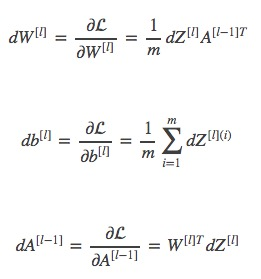
\includegraphics[width=12cm]  {8.jpg}}
 \caption{预测房屋价格}
 \label{fig:8}
\end{figure}

\subsection{Matrix Multiplication Properties 矩阵乘法的性质}
性质:
\begin{itemize}
  \item Let A and B be matrices.Then in general, A $\times$ B $\neq$ B $\times$ A.(not commutative)
  \item For any martix A,I is identity martix, A $\cdot$ I = I $\cdot$ A = A
  \item (A $\times$ B) $\times$ C = A $\times$ (B $\times$ C)
\end{itemize}

\subsection{Inverse and Transpose 逆、转置}
Matrix inverse:

\qquad If A is an m$\times$m matrix,and if it has an inverse,

 \qquad \qquad \qquad $AA^{-1}=A^{-1}A=I$

用Octave的软件求值:
\begin{itemize}
 \item 输入: A 3 4 2 16  得到矩阵A
 \item 输入:pinv(A) 得到矩阵A的逆矩阵的近似解
 \item 输入:inverseOFA=pinv(A) inverseOFA的值就是逆矩阵的近似解
\end{itemize}

注意,逆矩阵必须是方阵。逆矩阵不存在的矩阵,他的专有名词是奇异矩阵(singular)或者叫退化矩阵(degenerate)。因此零矩阵就是奇异矩阵。

Matrix Transpose:

\qquad Let A be an m $\times$ n matrix,and let $B=A^{T}$.

\qquad Then B is an n $\times$ m matrix,and $B_{ij}=A_{ji}$.
\end{document}













\end{document}
